%% LaTeX-Beamer template for KIT design
%% by Erik Burger, Christian Hammer
%% title picture by Klaus Krogmann
%%
%% version 2.1
%%
%% mostly compatible to KIT corporate design v2.0
%% http://intranet.kit.edu/gestaltungsrichtlinien.php
%%
%% Problems, bugs and comments to
%% burger@kit.edu

\documentclass[18pt]{beamer}

%% SLIDE FORMAT

% use 'beamerthemekit' for standard 4:3 ratio
% for widescreen slides (16:9), use 'beamerthemekitwide'

\usepackage{templates/beamerthemekit}
\usepackage[utf8]{inputenc}
% \usepackage{templates/beamerthemekitwide}

%% TikZ INTEGRATION

% use these packages for PCM symbols and UML classes
\usepackage{templates/tikzkit}
% \usepackage{templates/tikzuml}
\usepackage{listings}
\usepackage{tabulary}

\selectlanguage{ngerman}

\title[Treppenerkennung für einen treppensteigenden Roboter]{Treppenerkennung für einen treppensteigenden Roboter}
\subtitle{Projektpraktikum Robotik und Automation I (Software)}
\author{Maximilian Heß}

\institute{Institut für Anthropomatik und Robotik (IAR) - Intelligente Prozessautomation und Robotik (IPR)}

% Bibliography

\usepackage[citestyle=authoryear,bibstyle=numeric,hyperref,backend=biber]{biblatex}
\addbibresource{templates/example.bib}
\bibhang1em

\begin{document}

%title page
\begin{frame}
	\titlepage
\end{frame}

%table of contents
\begin{frame}{Übersicht}
	\tableofcontents
\end{frame}



\section{Motivation}

\begin{frame}{Motivation}
	\begin{itemize}
		\item Ziel: Finden und Kartografieren von Treppen
		\item Ermöglicht die Einführung von Ebenen in 2D-Karten
		\item Verknüpfung der Ebenen mittels Treppenmarkierungen
		\item Anwendungsbeispiel: Wegfindung über mehrere Stockwerke
	\end{itemize}
\end{frame}



\section{Hintergrund}

\subsection{Roboterplattform - HMMWV}
\begin{frame}{Roboterplattform - HMMWV}
	\begin{itemize}
		\item Hardwareausstattung Basisversion
		\begin{itemize}
			\item Sick LMS 100 (LiDAR) zum 2-dimensionalen Mappen und Lokalisieren
			\item Brix mit Intel Core 2 Duo..
			\item ATmega-basiertes Steuerinterface (Atmel ATmega 2560)
			\item WLAN-Router
		\end{itemize}
		\item Hardwareerweiterungen für die Treppenerkennung
		\begin{itemize}
			\item Schnellerer Brix mit Intel i5 vierter Generation für 3D-Berechnungen
			\item Asus Action Camera für 3D-Erfassung der Umgebung
		\end{itemize}
	\end{itemize}
\end{frame}

\begin{frame}{Roboterplattform - HMMWV}
	\begin{center}
		%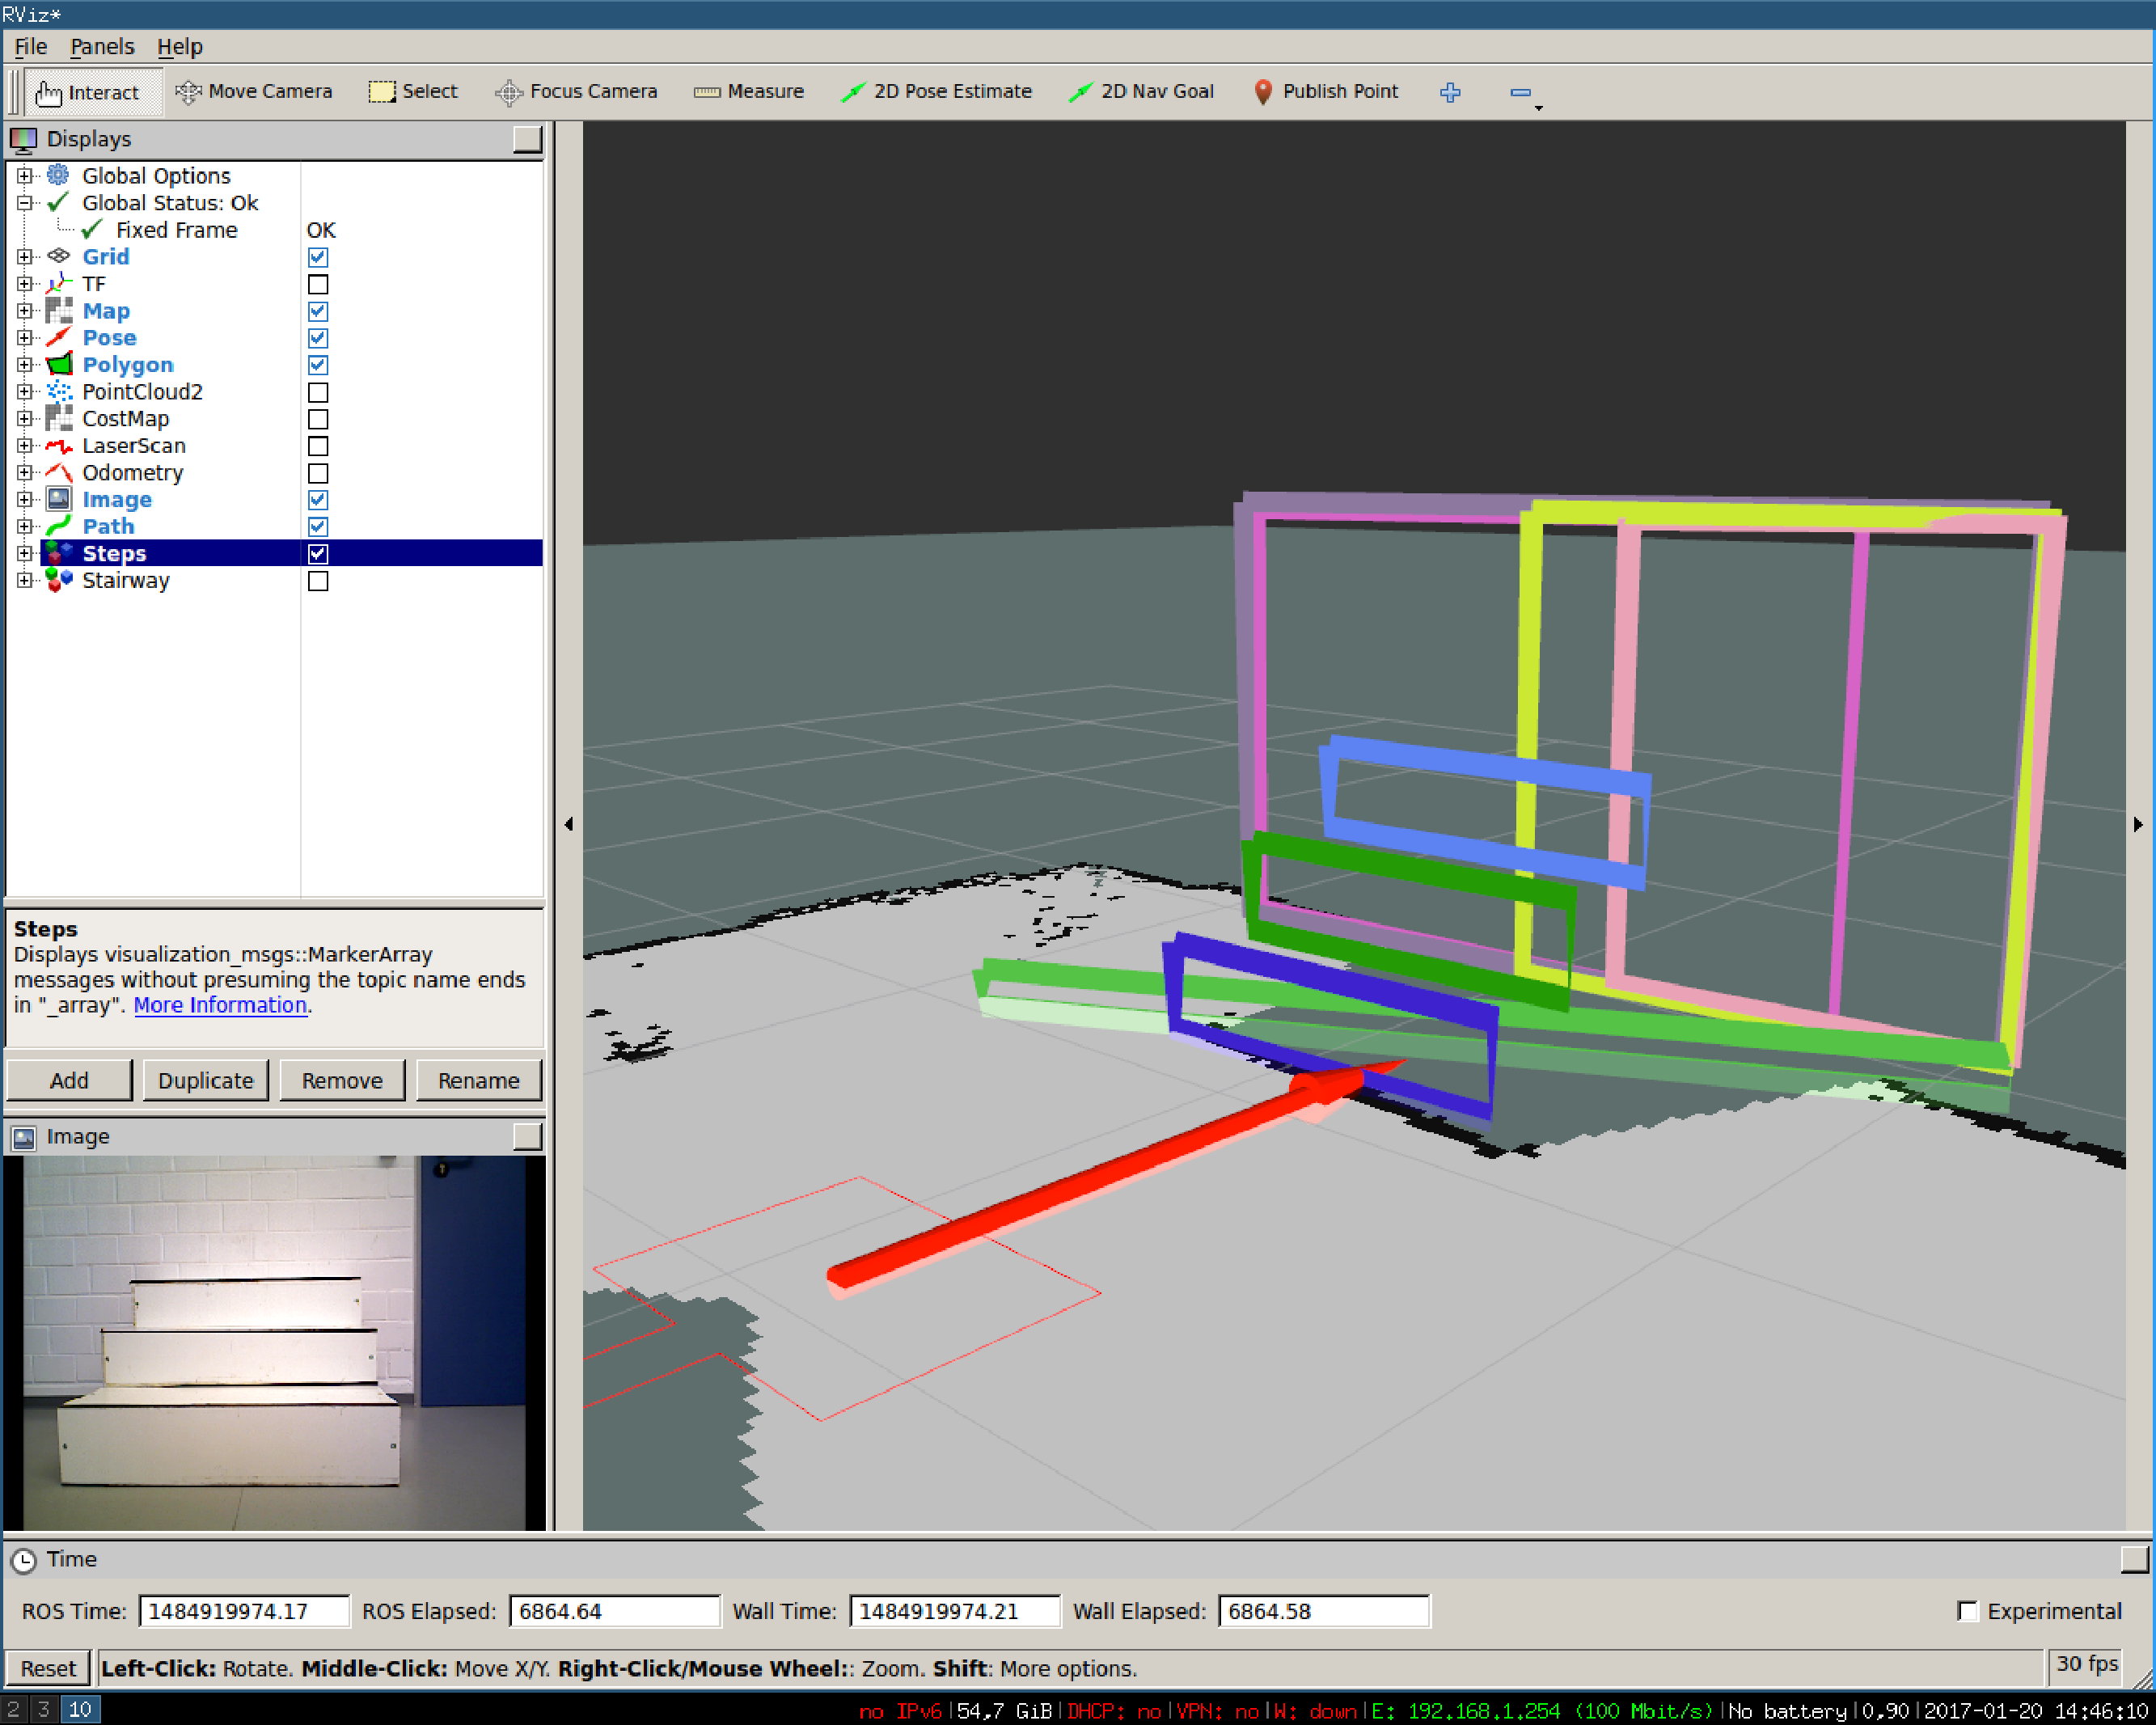
\includegraphics[scale=0.16]{images/ransac01.pdf}
		Foto von HMMWV
	\end{center}
\end{frame}


\subsection{Robot Operating System (ROS)}
\begin{frame}{Robot Operating System (ROS)}
	\begin{itemize}
		\item Verteilte Middleware zum Automatisieren von Kommunikation der Komponenten von Robotern
		\item Zentrale Aufgaben
		\begin{itemize}
			\item Nachrichtenaustausch zwischen Programmteilen
			\item Hardwareabstraktion
		\end{itemize}
		\item Viele Komponenten für Standardaufgaben (z.B. SLAM)
	\end{itemize}
\end{frame}

\begin{frame}{Node-Diagramm}
	\begin{center}
		%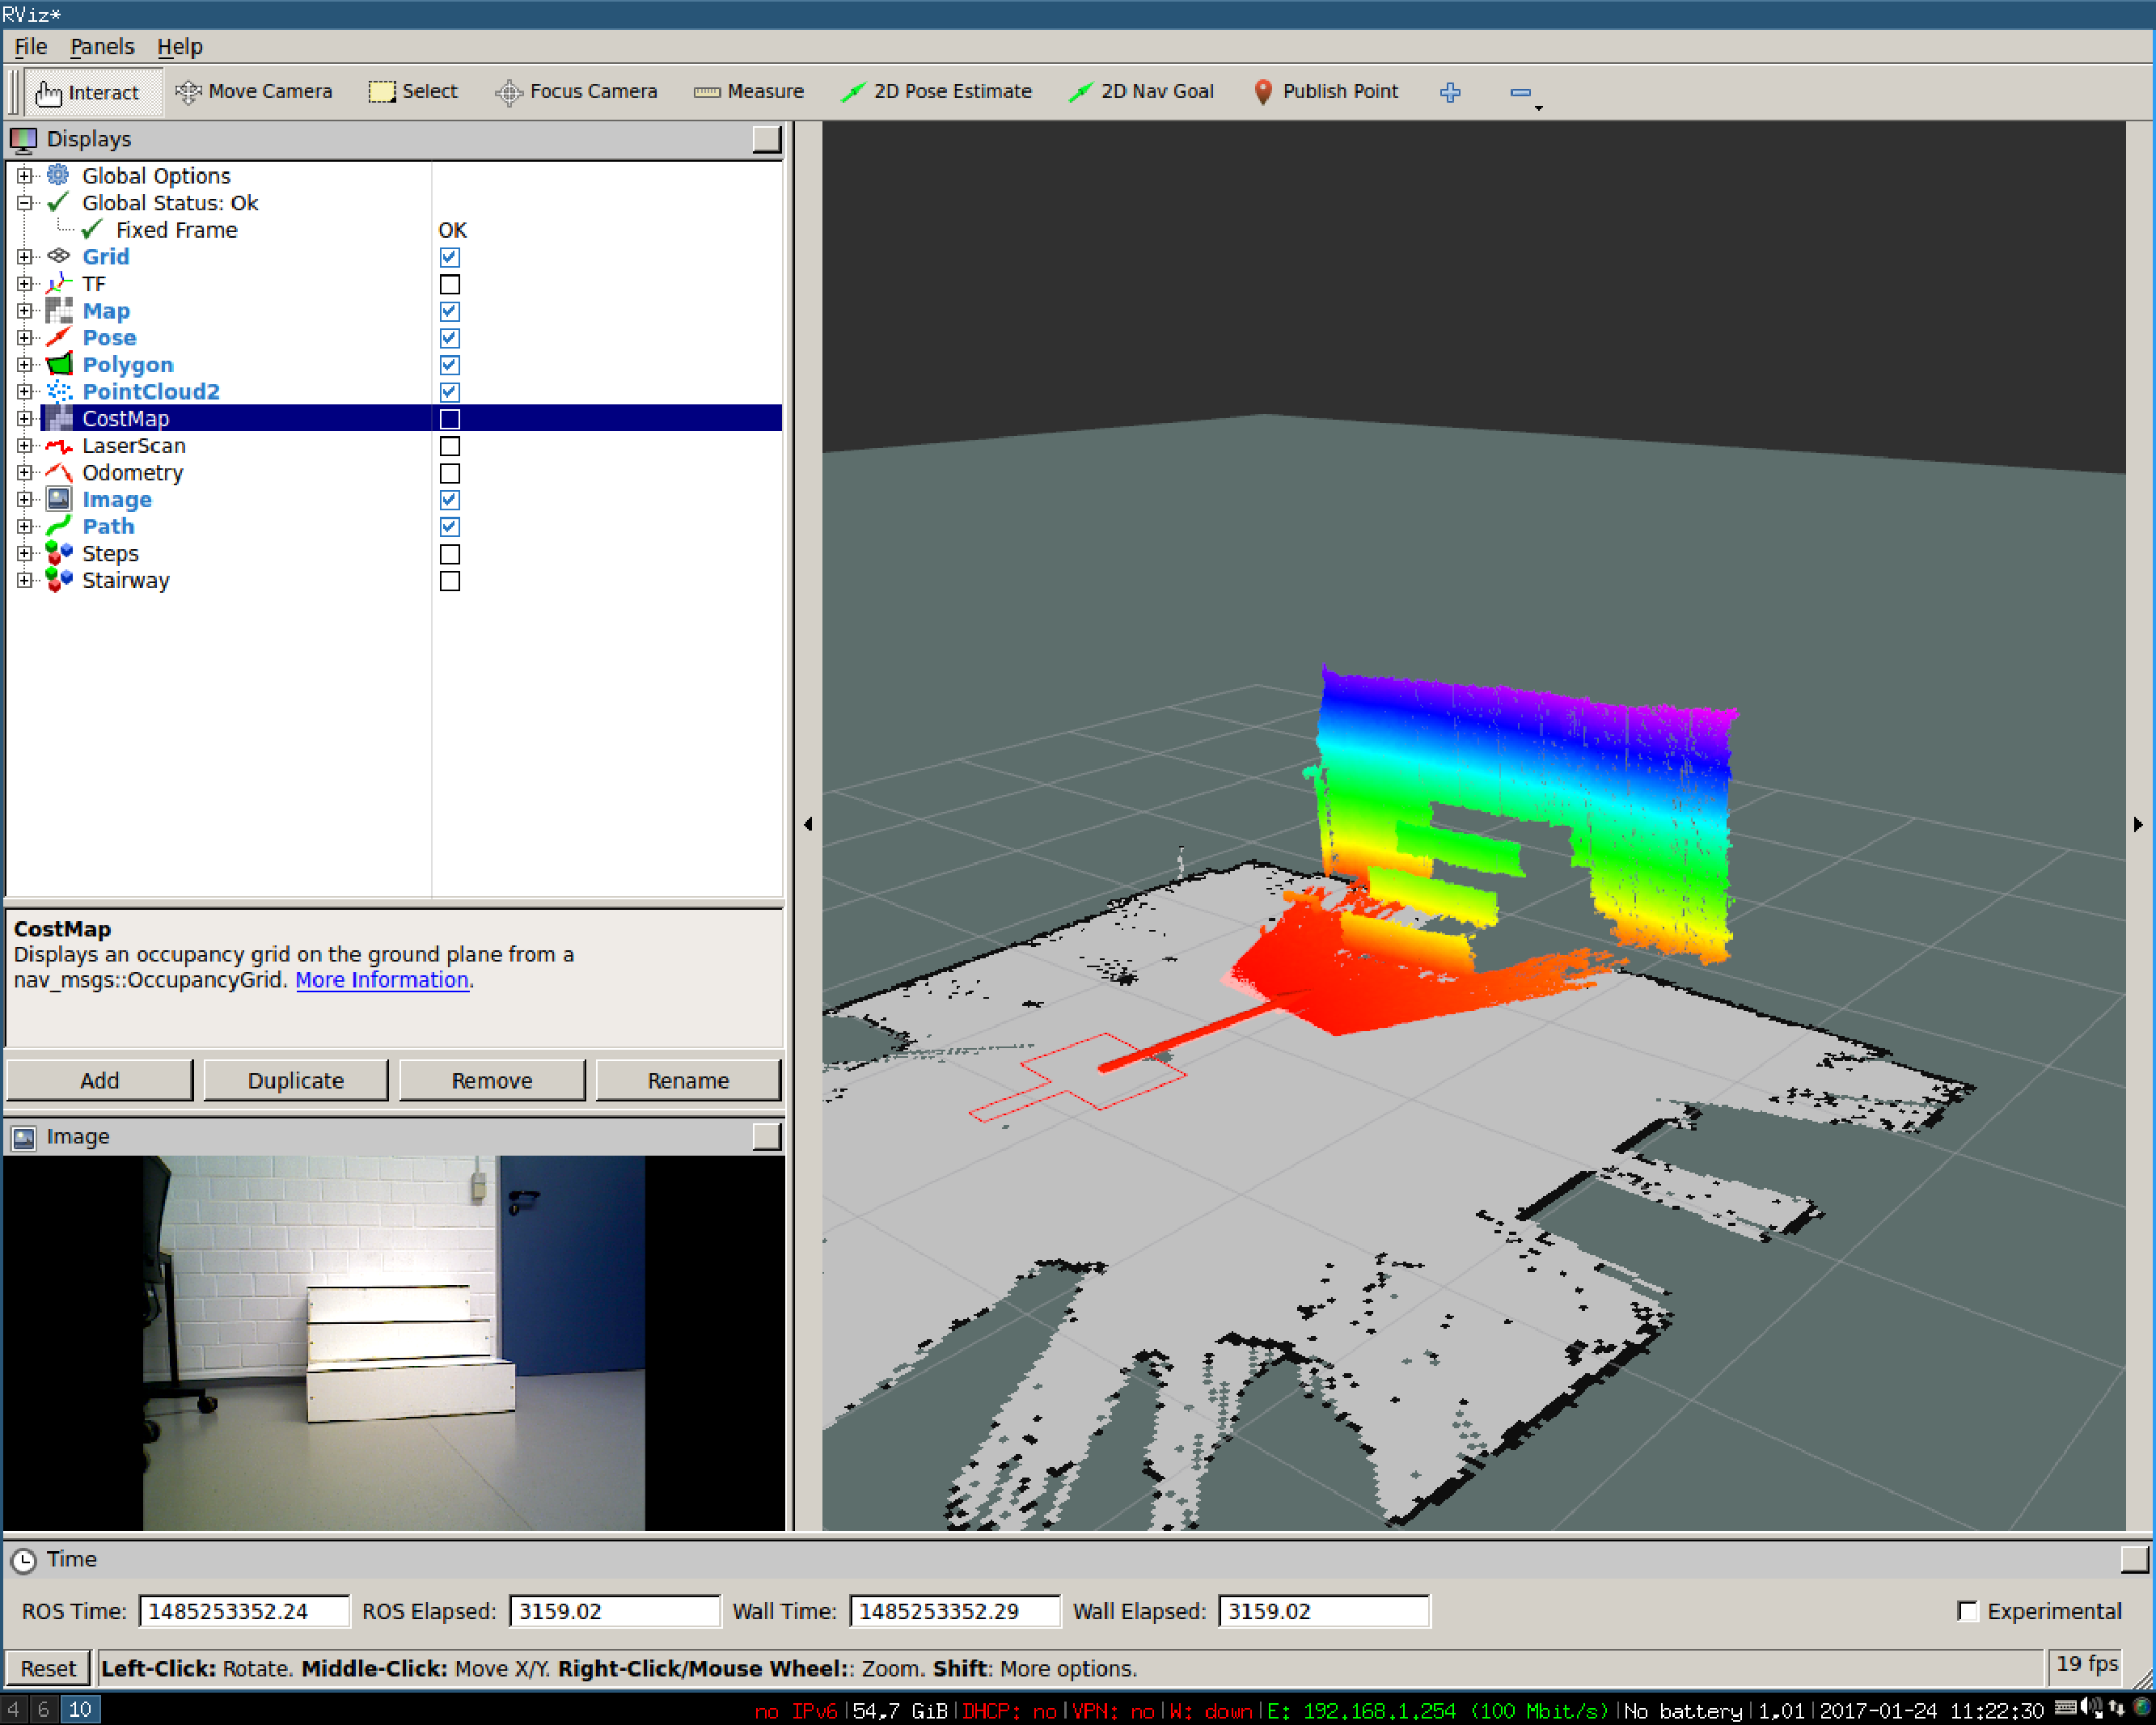
\includegraphics[scale=0.16]{images/ransac00.pdf}
		Turtlebot Diagramm
	\end{center}
\end{frame}



\section{Theoretische Vorüberlegungen}

\subsection{Ansatz 1: Erkennen von Treppen mittels horizontaler Linien }
\begin{frame}{Ansatz 1: Erkennen von Treppen mittels horizontaler Linien}
	\begin{itemize}
		\item Canny-Algorithmus zur Kantenerkennung
		\item Eingabe: Tiefenbild von Asus Xtion Kamera
	\end{itemize}
	\begin{columns}
		\column{0.25\textwidth}
		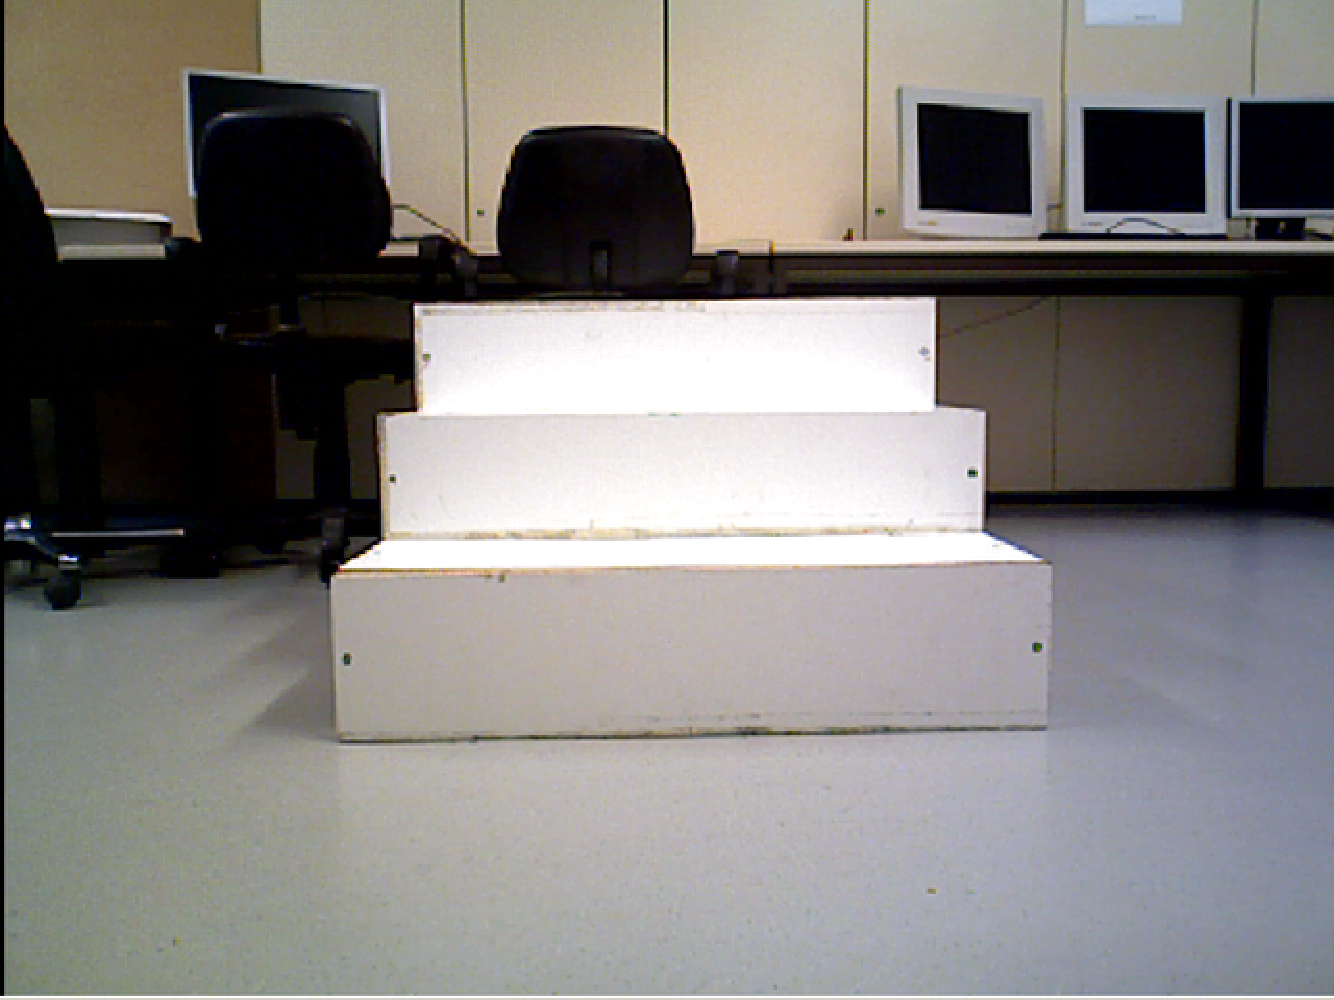
\includegraphics[scale=0.16]{images/canny00.pdf}\newline
		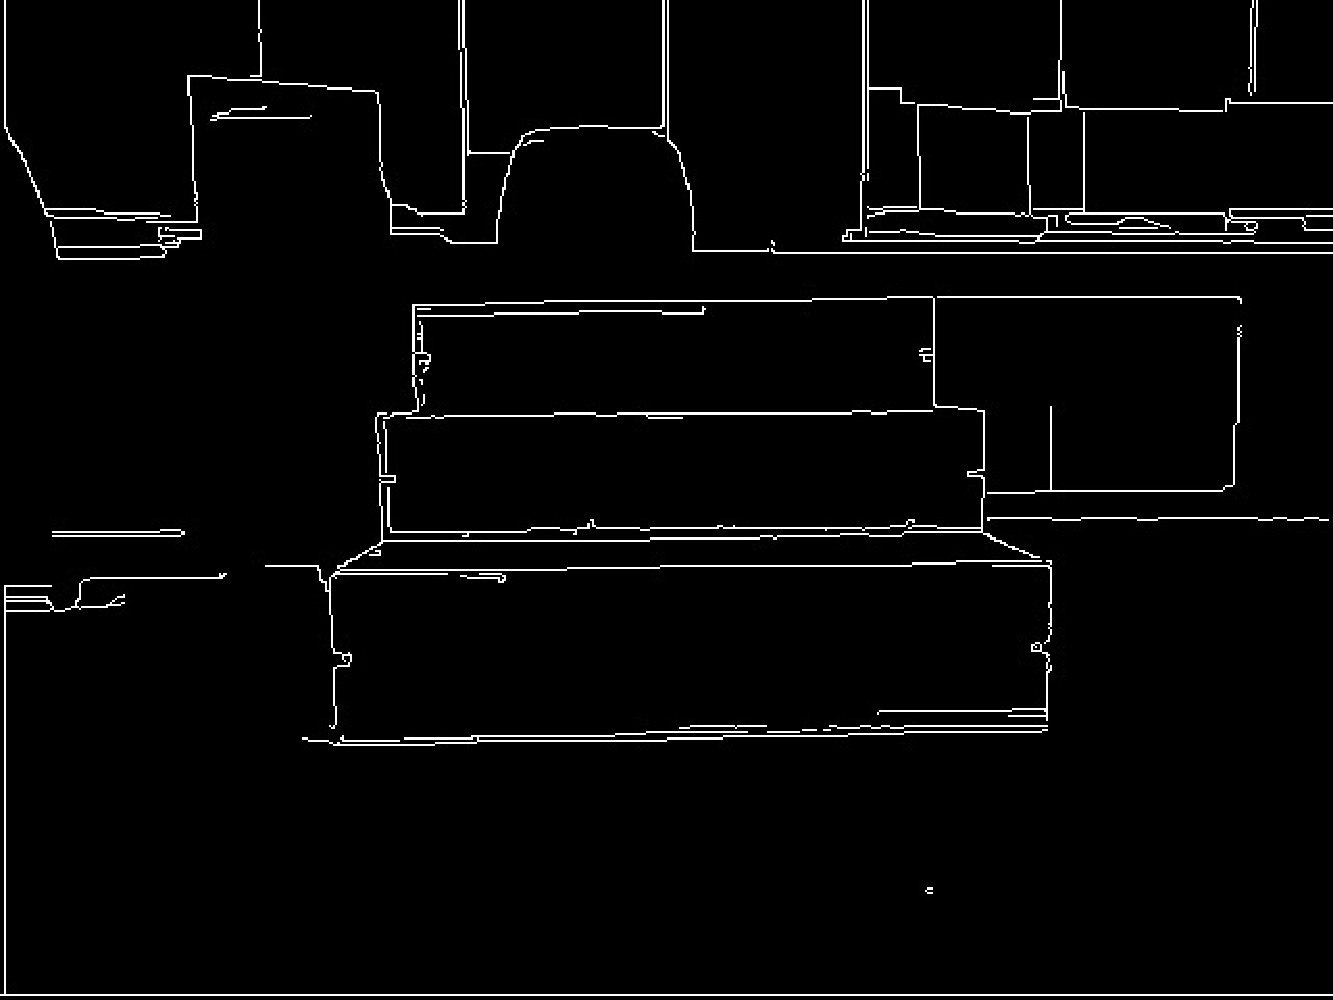
\includegraphics[scale=0.16]{images/canny02.pdf}
		\column{0.25\textwidth}
		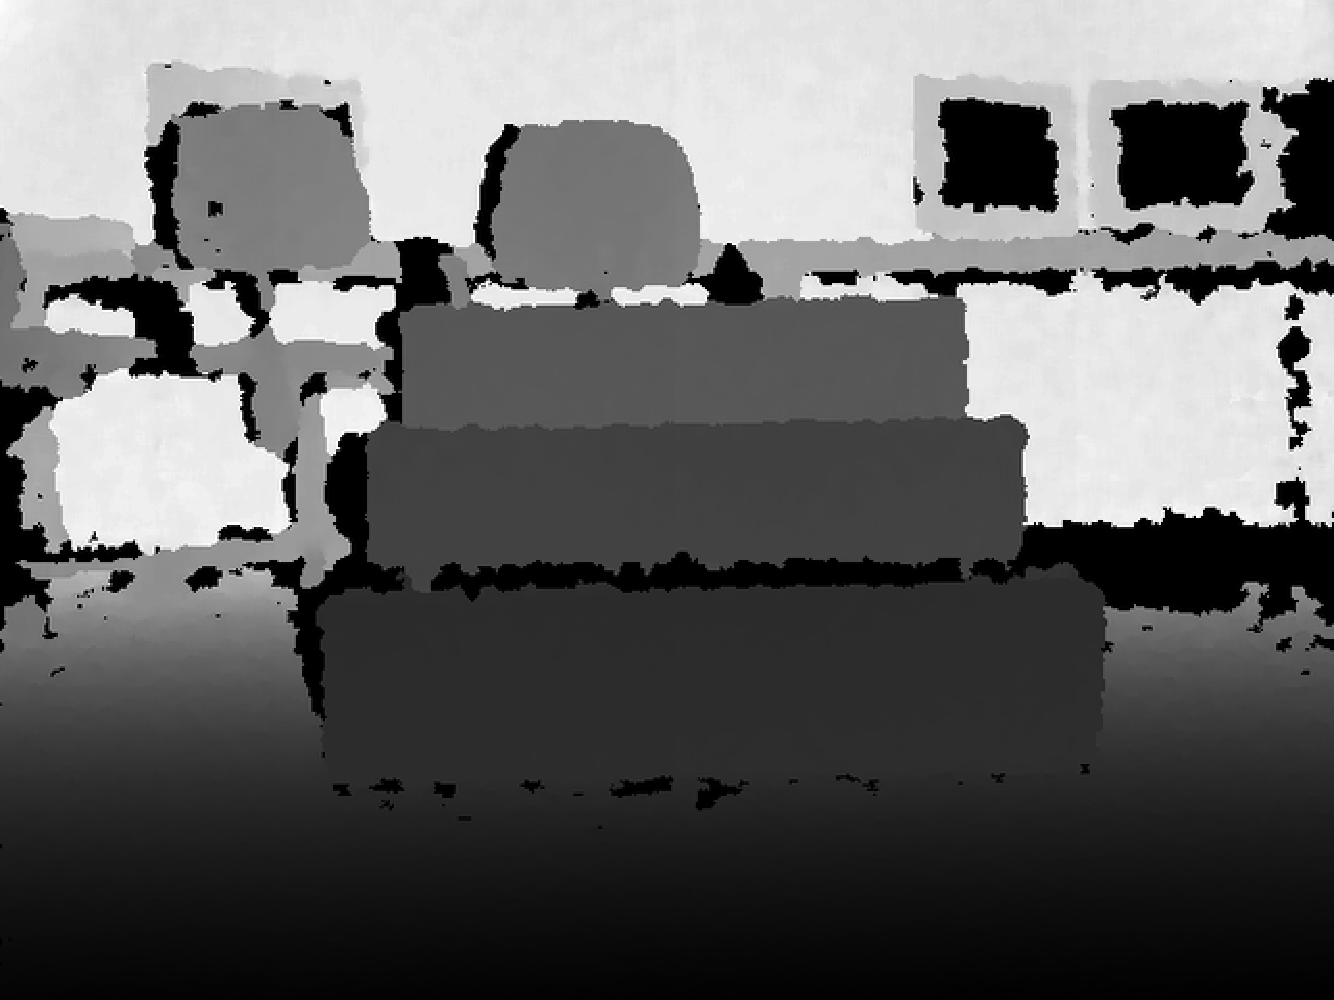
\includegraphics[scale=0.16]{images/canny01.pdf}\newline
		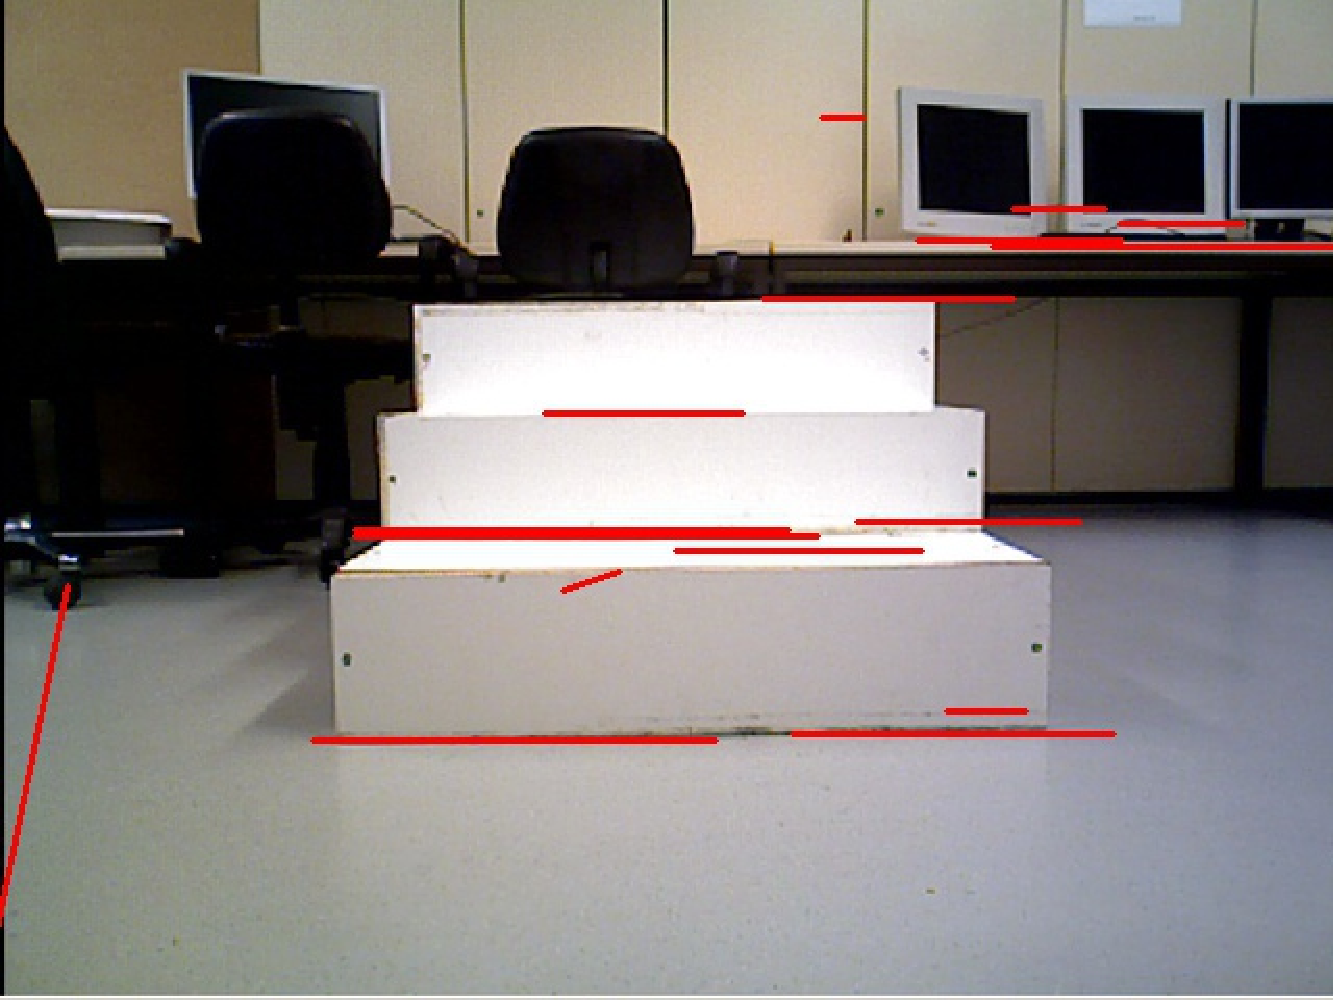
\includegraphics[scale=0.16]{images/canny03.pdf}
	\end{columns}
\end{frame}


\subsection{Ansatz 2: Erkennen von Treppen mittels vertikaler Flächen}
\begin{frame}{Ansatz 2: Erkennen von Treppen mittels vertikaler Flächen}
	\begin{itemize}
		\item Eingabe: zwei-dimensionale Punktwolke
		\item Verwendung des RANSAC-Algorithmus zur Ermittlung von Flächen (dazu gleich mehr)
	\end{itemize}
\end{frame}

\begin{frame}{RANSAC-Algorithmus}
	\begin{columns}
		\column{0.65\textwidth}
		\begin{itemize}
			\item Problem: Automatisch erfasste Messdaten enthalten meist viele Ausreißer
			\item RANSAC: Algorithmus zum Entfernen von Ausreißern \(\longrightarrow\) Ermittlung von Zwischenwerten
			\item Zwischenwerte als Eingabe für Zielalgorithmus
		\end{itemize}
		\column{0.35\textwidth}
		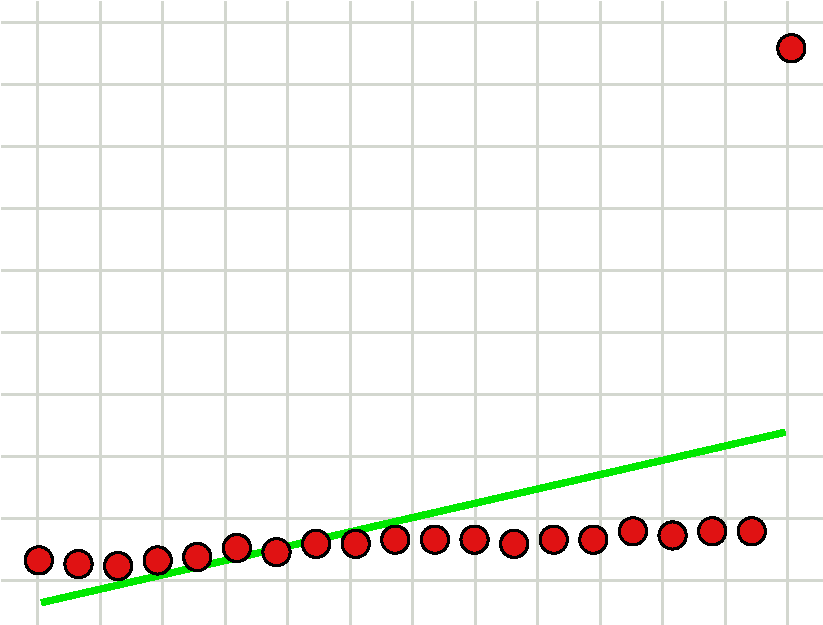
\includegraphics[scale=0.28]{images/ausreisser.pdf}
		(Quelle: Wikipedia)
	\end{columns}
\end{frame}



\section{Implementierung}

\begin{frame}{Implementierung}
	\begin{itemize}
		\item ROS Node zur Treppenerkennung
		\item C++, PCL
		\item Einführen Formats zur Speicherung der Treppen
		\begin{itemize}
			\item YAML
		\end{itemize}
		\item Import-/Export-Funktionen mittels \texttt{rosservice}
	\end{itemize}
\end{frame}

\begin{frame}{Implementierung im Detail}
	\begin{itemize}
		\item Eingabe: Punktwolke, Ausgabe: Treppenliste
	\end{itemize}
	\begin{center}
		\includegraphics[scale=0.42]{activitydiagram.pdf}
	\end{center}
\end{frame}

\begin{frame}{Implementierung im Detail}
	\begin{itemize}
		\item Nach Anwendung von \texttt{RANSAC}: Erkennen von senkrechten Flächen
	\end{itemize}
	\begin{center}
		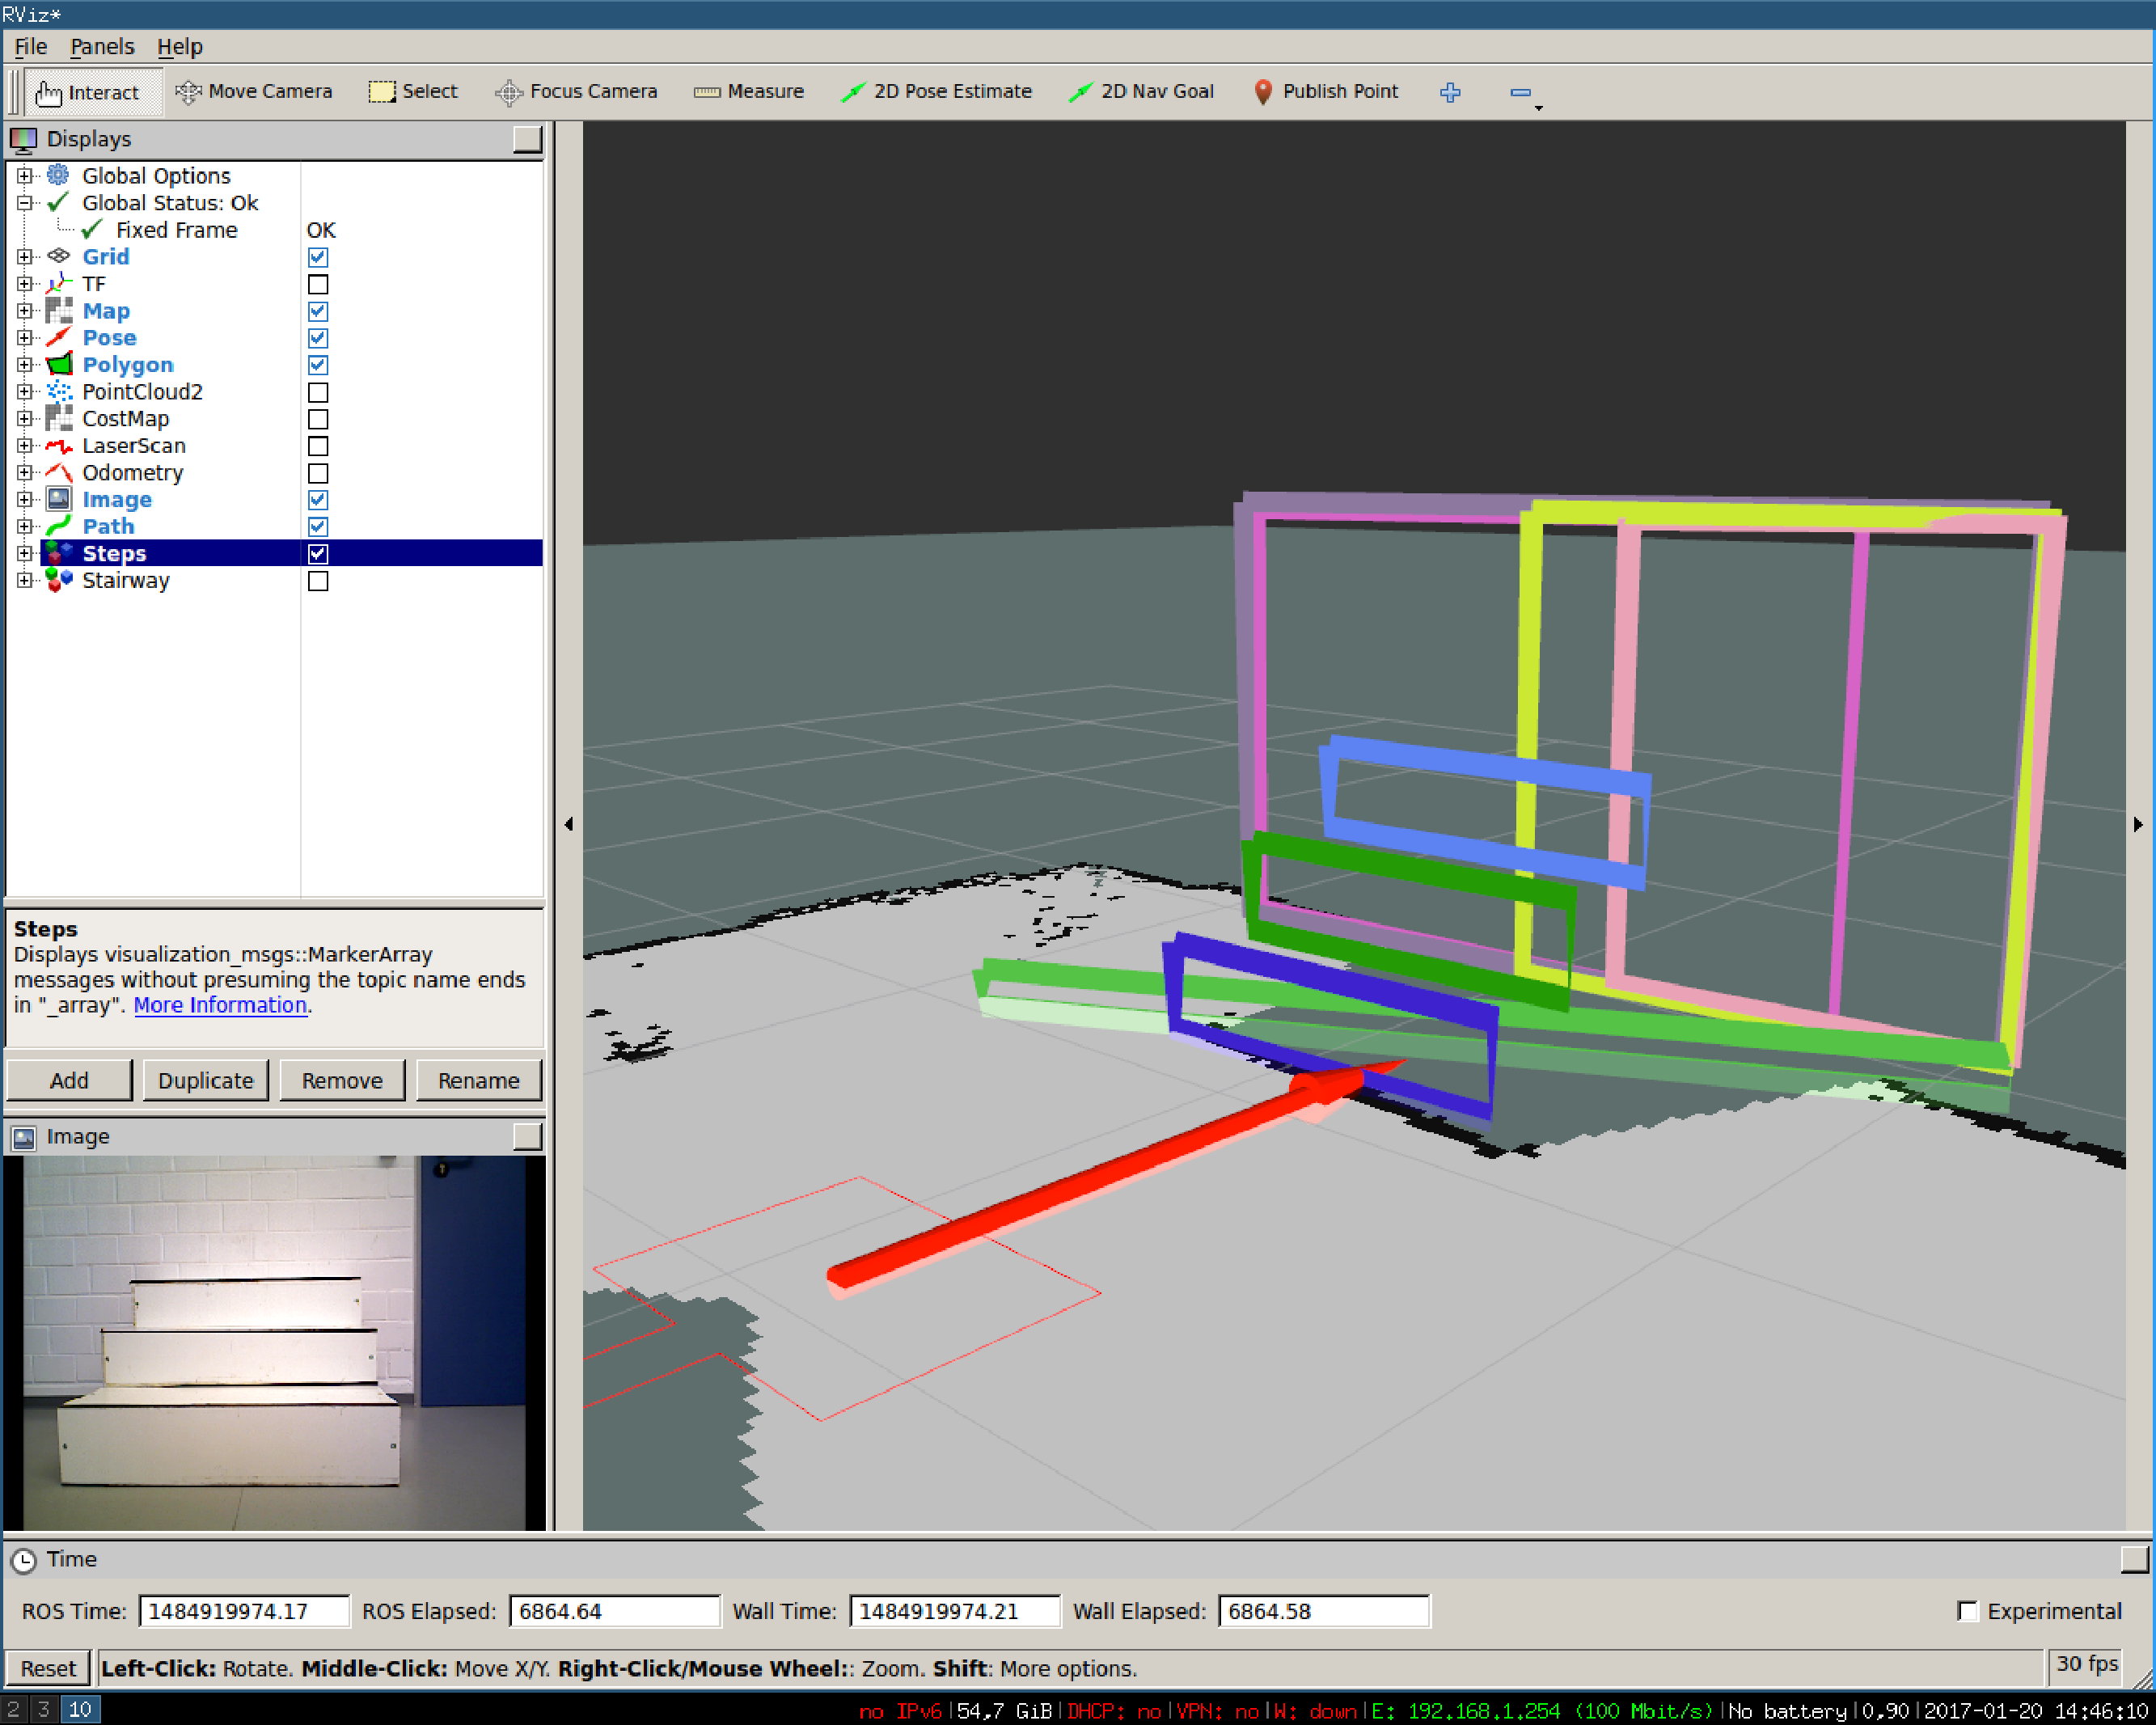
\includegraphics[scale=0.16]{images/ransac01.pdf}
	\end{center}
\end{frame}

\begin{frame}{Implementierung im Detail}
	\begin{itemize}
		\item Höhenfilter
	\end{itemize}
	\begin{center}
		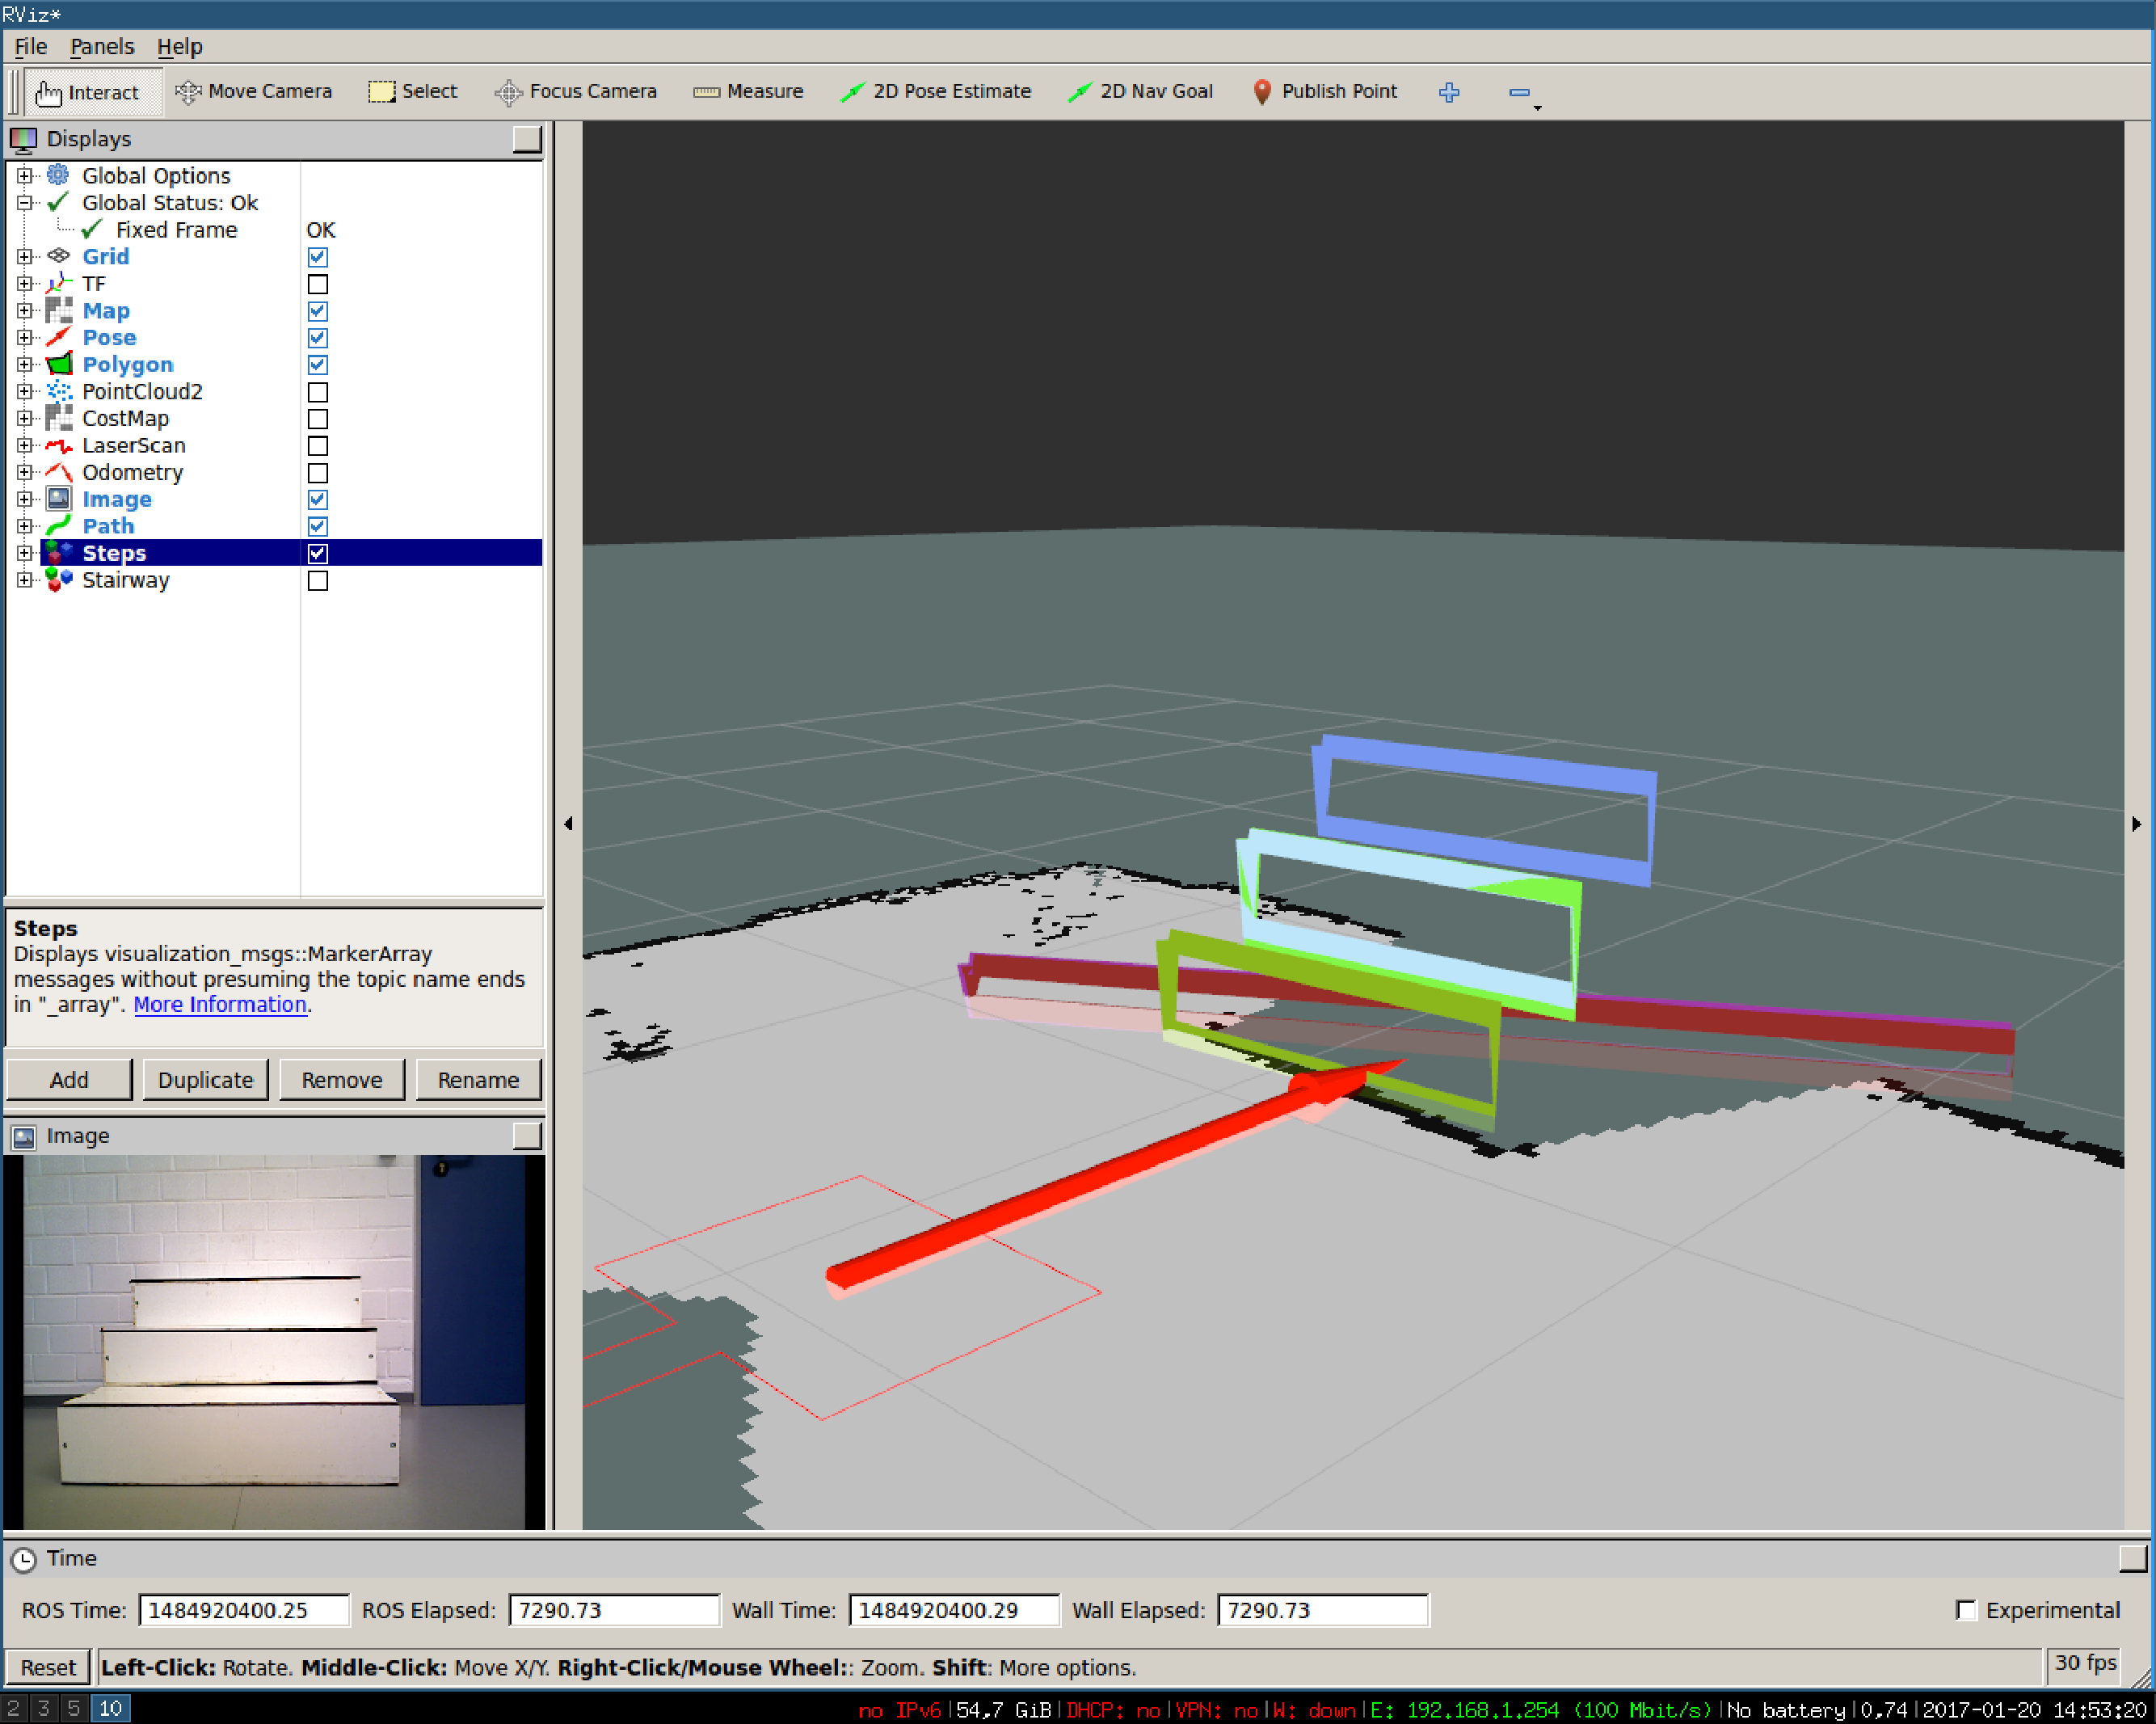
\includegraphics[scale=0.16]{images/ransac02.pdf}
	\end{center}
\end{frame}

\begin{frame}{Implementierung im Detail}
	\begin{itemize}
		\item Treppenbauen
	\end{itemize}
	\begin{center}
		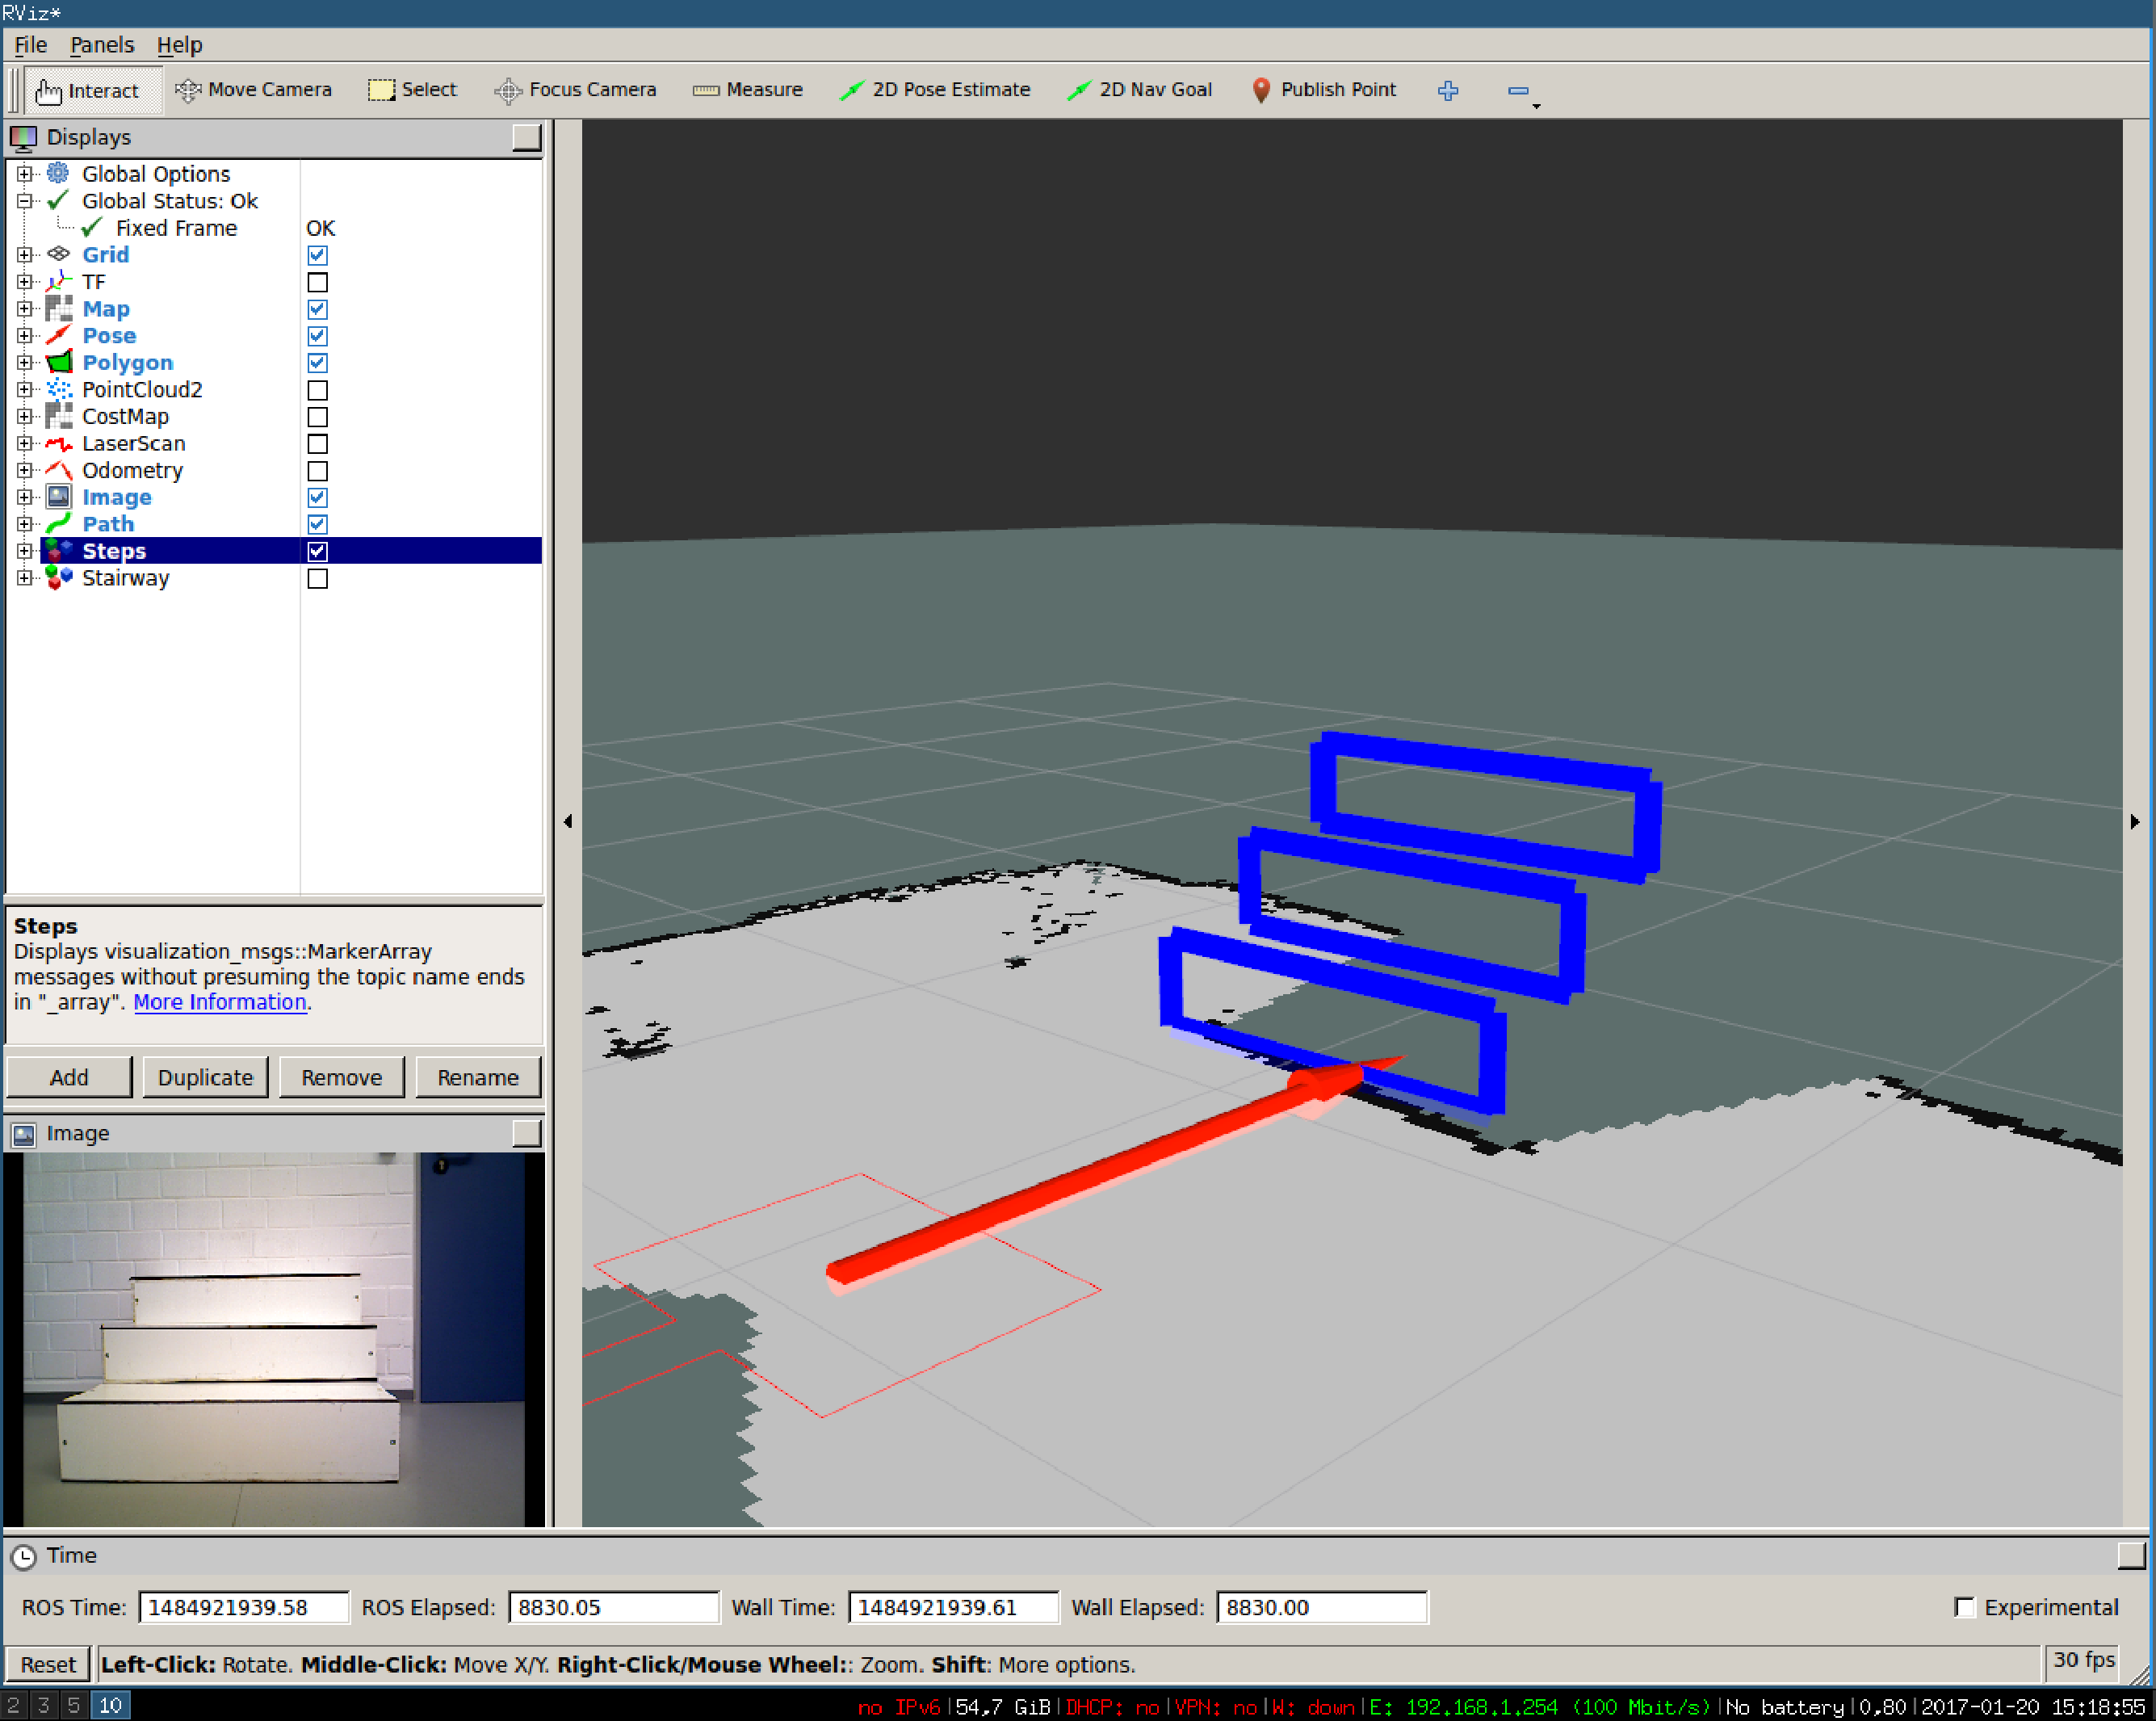
\includegraphics[scale=0.16]{images/ransac03.pdf}
	\end{center}
\end{frame}

\begin{frame}{Speicherformat für Import/Export}
	\begin{itemize}
		\item \texttt{rosservice call export\_stairways \~stairs.yaml}
	\end{itemize}

\end{frame}



\section{Bewertung des Ergebnisses}

\begin{frame}{Bewertung des Ergebnisses}
\begin{itemize}
	\item Beispieltreppe im Poolraum wird zuverlässig erkannt \(\longrightarrow\) Ziel erreicht
	\item Probleme/Schwächen
	\begin{itemize}
		\item Nur für sehr kurze Distanzen geeignet
		\begin{itemize}
			\item Kein Treppenmodell als Eingabe
			\item Reichweite der Kamera
		\end{itemize}
		\item Hohe Hardware-Anforderungen zur Verarbeitung der Punktwolken
	\end{itemize}
\end{itemize}
\end{frame}

\begin{frame}{Ausblick}
\begin{itemize}
	\item Langzeitvision: Verknüpfen mehrerer Kartenabschnitte durch Treppen
	\begin{itemize}
		\item Beispielsweise Stockwerke (eine Karte pro Stockwerk)
	\end{itemize}
	\item Einfügen eines geeigneten Treppenmodells
\end{itemize}
\end{frame}

\end{document}
